%% notes-tex/019-simb-multimodal-expression/sections/0-strand.tex
%% SOURCE: the expression, campaign and launch sections of the SIMB retrospective
%% (notes-tex/019-simb-multimodal/sections/2-expression.tex, 9-campaign.tex,
%% 10-launch.tex), carried over here so this document stands on its own. Every number
%% traces to the result file named beside it under experiments/019-simb-multimodal/results/
%% or to a named W&B run; the decoder-arm table is generated by decoder_arms_table.py.

\section{The strand before the campaign: task, model, and what was already known
\secstatus{todo}}
\label{sec:strand}

\subsection{The task and its ceiling\secstatus{todo}}
\label{sec:strand-task}

The \term{expression strand} predicts, for a strain carrying one gene deletion, the
$\log_2$ ratio of every measured gene's transcript abundance against wild type. Targets are
the Kemmeren 2014 knockout microarray compendium and the Sameith 2015 double-deletion
compendium (\path{doi:10.1016/j.cell.2014.02.054} and \path{doi:10.1038/sdata.2015.15}),
fused in the \file{fig3_core} build: 1{,}556 records, of which 1{,}484 are single deletions and 72 are
Sameith doubles, so $95.4\,\%$ of the training signal carries exactly one perturbed gene.
Every deleted gene appears exactly once, so under the strain-level partition no gene is in
both the fit and the validation split and every validation strain is an unseen
perturbation; a perturbation cannot be represented by its own observed response and must
enter through an external gene embedding.
\src{experiments/019-simb-multimodal/results/fig3_overlap_census.json}

The score is \file{pearson_per_feature}: for each reporter gene the Pearson correlation
across held-out strains between predicted and measured $\log_2$ ratio, averaged over
reporters. A model that predicts each gene's mean scores exactly zero on it, because a
prediction constant across strains has no variance to correlate; the companion per-strain
metric, \file{pearson_per_instance}, stays near $0.4$ under that same collapse and is the
form the perturbation-response literature reports (\cref{sec:strand-related}). The
\term{reproducibility ceiling} for the per-feature score is estimated from the 82 deletions
measured independently in both compendia, as the mean over reporters of
$\sqrt{\operatorname{clip}(\hat\rho_g, 0, 1)}$ with $\hat\rho_g$ the reporter's test-retest
correlation across the paired strains: $\mathbf{0.7746}$. The agreement between the two
studies' own measurements of those 82 deletions is $0.611$, which is the ceiling for any
cross-study statement.
\src{experiments/019-simb-multimodal/results/expression_ceiling_replicate.json}

\notesec{A third panel, and whether it measures the same thing} Nadal-Ribelles et al.\
2025 (doi:10.1038/s41467-025-57600-4) profiled about 3{,}100 single deletions of the same
collection by single-cell RNA-seq, pseudobulked per genotype against a wild type in the
same run, in base medium and under 0.4\,M NaCl; the base-medium records are 3{,}039
deletion ORFs, of which 914 are in Kemmeren and 44 in Sameith, and the union of the three
panels is 3{,}609 deletions against 1{,}484 today. Before that panel can extend the
perturbation axis it has to agree with the other two on the deletions they share, and
\cref{fig:cross-study} measures that with the same test-retest construction as the ceiling
above, on the base-medium records only.

The stored values need one correction first. They are scanpy \file{logfoldchanges} from
a Wilcoxon rank-sum call, a statistic that returns $\pm 23$ to $\pm 33$ whenever one
group's mean is zero; $20.3\,\%$ of the stored cells carry such a value and $22.6\,\%$ of
genes carry it in more than half of their records. Those cells are treated as absent.
What remains agrees with the microarrays on the deletions both measured almost not at
all: the per-strain profile correlation with Kemmeren has median $0.003$ over 914
deletions against $0.744$ for Kemmeren against Sameith over 82; the per-reporter
test-retest median is $0.030$ against $0.620$; the scale slope of Kemmeren on
Nadal-Ribelles is $0.006$ against $0.82$ on Sameith. On the reporters where Kemmeren's
effect exceeds one $\log_2$ unit the agreement is weak but above chance, median $0.10$
with signs agreeing $60\,\%$ of the time (chance $50\,\%$, the microarray pair
$93\,\%$), and the gene mapping is right: the cys3 deletion carries MET14, MET3 and MET6
up by $3$ to $3.7$ and CYS3 itself down, the induction that deletion is known for. The
paper's only comparison to Kemmeren is a count of genes at $p < 0.05$ over 837 shared
genotypes; it reports no profile correlation.
\src{experiments/028-knockout-expression/results/cross_study_ko_expression.json}

Two readings fit these numbers and the data here do not separate them: the per-genotype
pseudobulk is far noisier than a microarray replicate, or the Wilcoxon fold change is the
wrong statistic to have stored, or both. What separates them is a fold change recomputed
from the single-cell object (43\,GB on Zenodo, not in the raw mirror) as a pseudobulk
mean difference with a pseudocount and the paper's own mean-count filter, then the same
measurement again. Until that is done the panel cannot be pooled with the microarrays as
one target, since the two share neither a scale nor, on the shared deletions, an
ordering; its salt condition is a second environment of the same strains and a different
question.

\begin{figure}[htbp]
\centering
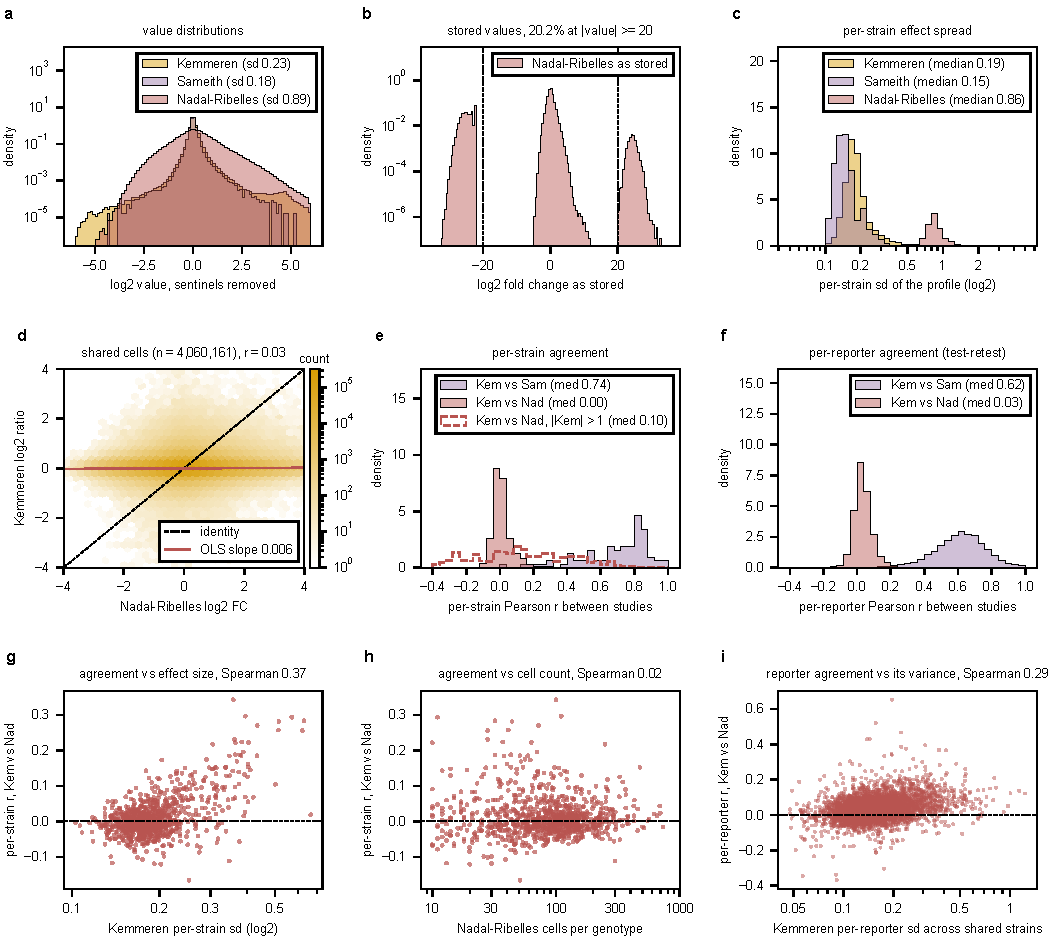
\includegraphics[width=\textwidth]{figures/cross_study_ko_expression.pdf}
\caption[]{Cross-study agreement of three single-deletion expression panels on the
deletions they share, base medium only, Nadal-Ribelles sentinel cells removed.
\textbf{a}, per shared deletion, the Pearson across reporter genes between its two
profiles (Kemmeren vs Nadal-Ribelles $n = 914$, Sameith vs Nadal-Ribelles $n = 44$,
Kemmeren vs Sameith $n = 82$); dashed, the same for Kemmeren vs Nadal-Ribelles over only
the reporters with $|\log_2| > 1$ in Kemmeren ($n = 368$ strains). \textbf{b}, per
reporter gene, the Pearson across shared strains between its two response vectors, the
test-retest reliability behind the ceiling. \textbf{c}, Kemmeren against Nadal-Ribelles on
every shared (strain, gene) cell, log-count density; the fitted slope is $0.006$.
Generated by \file{cross_study_ko_expression.py}.}
\label{fig:cross-study}
\end{figure}

\notesec{The byte count misleads} The compendium holds 9.2 million scalar labels against
0.39 million trigenic-interaction labels in the 010 queries, and the intuition that
expression would therefore be the easier task was wrong. In the trigenic data a gene recurs
across many records with different partners, so the supervision repeatedly constrains its
contribution; in the expression data a gene is the perturbation exactly once and is
measured on one array, so its 6{,}169 labels are 6{,}169 correlated readouts of a single
perturbation event and nothing in the data isolates the deletion's effect from the array's.
The perturbation axis has 1{,}484 points, and no objective or mechanism changes that.

\subsection{The model, and the one place strain identity enters\secstatus{todo}}
\label{sec:strand-model}

The incumbent is the equivariant cell-graph transformer
(\file{equivariant_cell_graph_transformer.py} under \file{torchcell/models/}): gene tokens from a frozen
embedding (\file{calm}) projected to width 90, a learnable CLS token prepended, six
encoder layers whose self-attention is hard-masked by the nine interaction graphs, then a
cross-attention \term{perturbation operator} whose keys are the deleted genes, then a
per-gene readout MLP shared across every gene token. The checkpoint's state dict
reconciles exactly to the logged parameter count.

\begin{table}[htbp]
\centering\small
%% SOURCE: results/launch_plan_evidence.json, param_count (1445-last.ckpt state dict,
%% deduplicated by tensor storage)
\begin{tabular}{lrl}
\toprule
module & parameters & role \\
\midrule
\file{transformer_layers} & 590{,}220 & 6 graph-masked encoder layers \\
\file{embedding_preprocessor} & 369{,}639 & input projection to $d = 90$ \\
\file{post_perturbation_mixing} & 101{,}430 & Perceiver mixing after the perturbation \\
\file{perturbation_transform} & 98{,}370 & the cross-attention perturbation operator \\
\file{perturbation_head} & 16{,}381 & graph-level scalar head \\
\file{per_gene_head} & 9{,}919 & per-gene readout, $d \to 19$ quantile knots \\
\file{observed_label_encoder} & 8{,}460 & masked teacher-forcing encoder \\
\file{cls_token} & 90 & \\
\midrule
total trainable & \textbf{1{,}194{,}509} & matches the logged \file{total_param_count} \\
\bottomrule
\end{tabular}
\caption[]{Parameter budget of the incumbent. The readout row is the striking one: 6{,}127
reporter genes are predicted by 9{,}919 parameters, because \file{PerGeneHead} is one MLP
shared across every gene token. The perturbation operator, at $8\,\%$ of the parameters,
carries the entire burden of making a prediction strain-specific.}
\label{tab:strand-params}
\end{table}

\pfstep{The encoder runs once, on the wild-type graph, and every strain reuses it} The
forward pass encodes the 6{,}607 gene tokens plus CLS once per batch, with no strain
information in the input; the batch dimension appears only at the perturbation operator,
which takes the shared gene states $H$ and each strain's deleted-gene indices. Two
consequences follow directly from the code. The CLS state $h_{\mathrm{CLS}}$ is
wild-type for every strain: measured across-strain standard deviation $0.0$ against
$0.973$ for the pooled perturbed-set summary $z_S$, so the conditioner input
$[z_S ; h_{\mathrm{CLS}}]$ carries strain identity in one half only, and the FiLM arm was
rewired to read $z_S$ alone because half its first-layer weights saw a constant. And the
perturbation never enters the graph-masked attention at all: the graphs shape how
wild-type gene states mix, and the deletion is applied to the finished states afterward.
\src{torchcell/models/equivariant_cell_graph_transformer.py (PerGeneHead construction and
the forward pass; the sd figures are recorded in the code comment there)}

\pfstep{At one deletion the operator has no pair term} The cross-attention's softmax runs
over a key set of size one, so its weight is identically 1. Re-drawing $W_Q$ and $W_K$ at
standard deviation 10 changes the output by exactly $0.0$, and 16{,}200 of the operator's
32{,}760 attention parameters are dead at $|S_b| = 1$. The model therefore reduces to
$g(h_i + c_b)$: reporter identity $i$ and strain identity $b$ meet once, by addition, and no
term depends on the pair (deleted gene, reporter gene). Masked unmasking does not supply
one where the score is taken: at reveal step $k = 0$ every mask bit is zero, the
conditioning branch's inputs are zero as inputs, and the forward pass is identical to the
unconditioned model.
\src{experiments/019-simb-multimodal/results/perturbation_selector_degeneracy.json}

\begin{table}[htbp]
\centering\small
%% SOURCE: torchcell/models/equivariant_cell_graph_transformer.py (mechanisms and ranks
%% from the module docstrings and init code); the derivation is in
%% notes/experiments.019-simb-multimodal.multiplicative-perturbation-conditioning.md
\begin{tabular}{llp{62mm}}
\toprule
mechanism & pair rank & how one deletion reaches many genes \\
\midrule
additive reference & 0 & it does not: one $c_b$ added to every gene \\
null sink & 9 & sigmoid gate per head, $\alpha_i$ depends on the querying gene \\
graph propagation & data & random-walk mass from the deleted gene over the nine graphs, plus a hop-0 self indicator \\
low-rank bilinear & $r$ & $\sum_j b_{ij}(h_i)\, a_j(c_b)$ \\
response basis & $r$ & factored readout, $r$ shared response directions \\
GEARS-style cross-gene & $r$ & pool over genes, low-rank broadcast back, in the decoder \\
per-gene readout & -- & one output weight per reporter, as GEARS and State have \\
Hadamard / FiLM & 90 & $h_i \odot (1 + \gamma(c_b))$, gene and strain multiply \\
\bottomrule
\end{tabular}
\caption[]{Pair-term mechanisms resident in the model file, each gated to be the exact
identity at initialization and selectable by config. The rank is what each can express,
a derivation and not a measurement; which have been trained, and at what budget, is
\cref{sec:strand-heads} and \cref{sec:readouts-mech}.}
\label{tab:strand-pair-rank}
\end{table}

\pfstep{Rank is not what binds} The best rank-$r$ approximation of the
$1{,}482 \times 6{,}169$ target matrix, scored with the same per-feature Pearson on the
matrix it was fit to, reaches $0.7265$ at rank 32 and $0.7799$ at rank 64, both at the
ceiling. A rank-64 pair term has expressive room by a wide margin, so a null from such an
arm is about the mechanism or the optimization and not about capacity. After removing each
gene's mean, the residual gene-gene correlation pattern replicates on held-out strains at
split-half $r = 0.8687$ against a permutation null of $8.5 \times 10^{-5}$, with effective
rank $32.78$; that structure is the reason a per-gene independent readout, which emits
6{,}169 separate marginals, discards most of what the data hold.
\src{experiments/019-simb-multimodal/results/lowrank_output_ceiling.json}
\src{experiments/019-simb-multimodal/results/residual_covariance_diagnostic.json}

\subsection{Heads and decoder families already trained\secstatus{todo}}
\label{sec:strand-heads}

Two comparisons are on record from before the campaign, and neither is a comparison.

\pfstep{Six distributional heads, five of them never past 200 epochs} The incumbent's
quantile head rests on the table below, read from the leaderboard as it stood when the
campaign was designed.

\begin{table}[htbp]
\centering\small
%% SOURCE: results/round_leaderboards.csv as read on 2026-08-31 for the SIMB retrospective
%% (expression + expression_masked strands); reproduced here unchanged.
\begin{tabular}{lrrrrr}
\toprule
 & \multicolumn{3}{c}{all runs} & \multicolumn{2}{c}{matched budget, 100--200 epochs} \\
\cmidrule(lr){2-4}\cmidrule(lr){5-6}
\file{dist} head & runs & best & max epochs & best & median \\
\midrule
\file{quantile}     & 344 & $0.2382$ & 9{,}900 & $0.1751$ & $0.1352$ \\
\file{crps}         & 158 & $0.1631$ & 199 & $0.1631$ & $0.1267$ \\
\file{energy}       &  50 & $0.1421$ & 199 & $0.1421$ & $0.0960$ \\
\file{laplace_crps} &  56 & $0.1411$ & 199 & $0.1411$ & $0.0775$ \\
\file{point}        &  34 & $0.1117$ & 163 & $0.1117$ & $0.1054$ \\
\file{nll}          &  59 & $0.0983$ & 199 & $0.0845$ & $0.0680$ \\
\bottomrule
\end{tabular}
\caption[]{The head comparison the incumbent rested on, before the objective round. The
left block compares one head at 9{,}900 epochs against five at about 150; the right block
is the window where all six ran, on which \file{quantile} leads by $0.0085$ on the median
with its maximum drawn from 84 runs against \file{crps}'s 25. \file{nll} is the designed
$\sigma$-collapse control; \file{energy}'s covariance is global and cannot move a point
metric. The objective round (\cref{sec:findings-head}) is what replaced this table.}
\label{tab:strand-dist-confound}
\end{table}

\pfstep{The decoder and perturbation families, all inside the early dip} The GEARS-style
cross-gene readout, the rank-32 bilinear pair term, Perceiver post-perturbation mixing, the
rank-32 response basis, context concatenation, graph propagation, the null sink and the
deeper perturbation heads were each trained in waves 1 to 3 of project
\file{torchcell_019_expr_v8}, most at one seed (\cref{tab:decoder-arms-v8}). Sixty-seven
scored runs across waves 1 to 4b, and not one ran past 300 epochs, against a validation
curve that dips at epochs 200 to 300 and then climbs for thousands more
(\cref{sec:findings-lossmin}). Every one of them was stopped inside the dip, so the
differences between arms are early-training transients and more seeds at that budget buy
precision on the wrong estimand. Of the families in the table, only two have since been
trained at a resolving budget: the rank-64 response basis and the per-gene readout, as the
mechanism round (\cref{sec:readouts-mech}). The GEARS-style cross-gene readout, the
bilinear term, Perceiver mixing on its own and FiLM have not been.

%% GENERATED by experiments/019-simb-multimodal/scripts/decoder_arms_table.py
%% from results/decoder_arms_torchcell_019_expr_v8.csv (score_decoder_arms.py) and
%% the arm overrides in scripts/gh_expr_008_arm.sh. Do not edit by hand.
%% SOURCE: the two files named above.
\begin{table}[htbp]
  \centering
  \footnotesize
  \caption[Decoder and perturbation-family arms of the v8 round]{The decoder and perturbation-family arms of waves 1 to 3 in project \file{torchcell_019_expr_v8}, 35 runs over 21 arm-wave cells, scored by the maximum of a centered 5-epoch rolling mean of the validation Pearson (\file{score_decoder_arms.py}). Every run stopped between epochs 50 and 276, inside the early dip of a curve that is still rising at 9{,}900 (\cref{sec:findings-lossmin}), so the scores measure early-training transients and the column is not an arm comparison. The GEARS-style cross-gene readout, the bilinear pair term, Perceiver mixing and the response basis are all here, each at one seed. The mechanism column is a gloss on the override, which is the launcher's own text.}
  \label{tab:decoder-arms-v8}
  \begin{tabular}{@{}ll>{\raggedright\arraybackslash}p{0.30\textwidth}rrr@{}}
    \hline
    Arm & Wave & Mechanism (override) & Seeds & Epochs & Smoothed max, mean / best \\
    \hline
    \texttt{A0\_baseline} & 1 & additive reference, $g(h_i + c_b)$ (\texttt{\scriptsize none}) & 3 & 80--120 & $0.081$ / $0.153$ \\
    \texttt{A1\_free16} & 1 & free per-gene lookup of 16 dims (\texttt{\scriptsize multitask.\allowbreak{}free\_gene\_dim=\allowbreak{}16}) & 1 & 139 & $0.152$ / $0.152$ \\
    \texttt{A2\_self} & 1 & self-indicator only (hop 0) (\texttt{\scriptsize "\$PROP=\allowbreak{}true" model.\allowbreak{}perturbation\_propagation.\allowbreak{}hops=\allowbreak{}0}) & 1 & 123 & $0.152$ / $0.152$ \\
    \texttt{A4\_prop\_h2} & 1 & random-walk propagation, 2 hops (\texttt{\scriptsize "\$PROP=\allowbreak{}true" model.\allowbreak{}perturbation\_propagation.\allowbreak{}hops=\allowbreak{}2}) & 3 & 70--140 & $0.100$ / $0.172$ \\
    \texttt{A6\_prop\_sparse} & 1 & propagation, 2 hops, sparse (\texttt{\scriptsize "\$PROP=\allowbreak{}true" model.\allowbreak{}perturbation\_propagation.\allowbreak{}hops=\allowbreak{}2 "model.\allowbreak{}perturbation\_propagation.\allowbreak{}graphs=\allowbreak{}[\allowbreak{}regulatory\_interaction,\allowbreak{}tflink,\allowbreak{}physical\_interaction]"}) & 1 & 140 & $0.175$ / $0.175$ \\
    \texttt{B0\_protT5} & 1 & ProtT5 gene embeddings (\texttt{\scriptsize "cell\_dataset.\allowbreak{}node\_embeddings=\allowbreak{}[\allowbreak{}prot\_T5\_all]"}) & 1 & 70 & $0.089$ / $0.089$ \\
    \texttt{A6\_prop\_sparse} & 2 & propagation, 2 hops, sparse (\texttt{\scriptsize "\$PROP=\allowbreak{}true" model.\allowbreak{}perturbation\_propagation.\allowbreak{}hops=\allowbreak{}2 "model.\allowbreak{}perturbation\_propagation.\allowbreak{}graphs=\allowbreak{}[\allowbreak{}regulatory\_interaction,\allowbreak{}tflink,\allowbreak{}physical\_interaction]"}) & 2 & 76--88 & $0.068$ / $0.090$ \\
    \texttt{C0\_concat} & 2 & head sees $[h_{\mathrm{pert}}; h_i; c_b]$ (\texttt{\scriptsize multitask.\allowbreak{}concat\_context=\allowbreak{}true}) & 1 & 140 & $0.161$ / $0.161$ \\
    \texttt{D1\_bilinear32} & 2 & rank-32 bilinear pair term (\texttt{\scriptsize multitask.\allowbreak{}bilinear\_rank=\allowbreak{}32}) & 1 & 123 & $0.152$ / $0.152$ \\
    \texttt{E0\_perceiver32} & 2 & Perceiver mixing after the perturbation (\texttt{\scriptsize model.\allowbreak{}post\_perturbation\_mixing.\allowbreak{}enabled=\allowbreak{}true model.\allowbreak{}post\_perturbation\_mixing.\allowbreak{}num\_latents=\allowbreak{}32}) & 1 & 114 & $0.157$ / $0.157$ \\
    \texttt{A0\_baseline} & 3 & additive reference, $g(h_i + c_b)$ (\texttt{\scriptsize none}) & 1 & 196 & $0.158$ / $0.158$ \\
    \texttt{A1\_ref} & 3 & additive reference, $g(h_i + c_b)$ (\texttt{\scriptsize none}) & 4 & 242--250 & $0.076$ / $0.158$ \\
    \texttt{A2\_prop\_sparse} & 3 & propagation, 2 hops, sparse (\texttt{\scriptsize "\$PROP=\allowbreak{}true" model.\allowbreak{}perturbation\_propagation.\allowbreak{}hops=\allowbreak{}2 "model.\allowbreak{}perturbation\_propagation.\allowbreak{}graphs=\allowbreak{}[\allowbreak{}regulatory\_interaction,\allowbreak{}tflink,\allowbreak{}physical\_interaction]"}) & 4 & 50--51 & $0.079$ / $0.130$ \\
    \texttt{A4\_nullsink} & 3 & null-sink gated attention (\texttt{\scriptsize model.\allowbreak{}perturbation\_head.\allowbreak{}null\_sink=\allowbreak{}true model.\allowbreak{}perturbation\_head.\allowbreak{}null\_sink\_bias\_init=\allowbreak{}-4.\allowbreak{}0 model.\allowbreak{}perturbation\_head.\allowbreak{}null\_sink\_trainable=\allowbreak{}true}) & 4 & 186--189 & $0.076$ / $0.149$ \\
    \texttt{D1\_bilinear32} & 3 & rank-32 bilinear pair term (\texttt{\scriptsize multitask.\allowbreak{}bilinear\_rank=\allowbreak{}32}) & 1 & 175 & $0.148$ / $0.148$ \\
    \texttt{D2\_mask} & 3 & hard graph mask replaces the KL (\texttt{\scriptsize model.\allowbreak{}attention\_mask.\allowbreak{}enabled=\allowbreak{}true model.\allowbreak{}graph\_regularization.\allowbreak{}graph\_reg\_lambda=\allowbreak{}0.\allowbreak{}0}) & 1 & 235 & $0.149$ / $0.149$ \\
    \texttt{E0\_perceiver\_on} & 3 & Perceiver mixing after the perturbation (\texttt{\scriptsize model.\allowbreak{}post\_perturbation\_mixing.\allowbreak{}enabled=\allowbreak{}true model.\allowbreak{}post\_perturbation\_mixing.\allowbreak{}num\_latents=\allowbreak{}32 'model.\allowbreak{}post\_perturbation\_mixing.\allowbreak{}gate\_mode=\allowbreak{}on'}) & 1 & 181 & $0.127$ / $0.127$ \\
    \texttt{F1\_attn4} & 3 & deeper perturbation head (\texttt{\scriptsize model.\allowbreak{}perturbation\_head.\allowbreak{}num\_layers=\allowbreak{}4 model.\allowbreak{}perturbation\_head.\allowbreak{}extra\_layer\_ffn\_mult=\allowbreak{}0}) & 1 & 222 & $0.155$ / $0.155$ \\
    \texttt{F1\_deep2} & 3 & deeper perturbation head (\texttt{\scriptsize model.\allowbreak{}perturbation\_head.\allowbreak{}num\_layers=\allowbreak{}2}) & 1 & 202 & $0.168$ / $0.168$ \\
    \texttt{GEARS\_crossgene} & 3 & GEARS-style cross-gene readout, rank 64 (\texttt{\scriptsize model.\allowbreak{}cross\_gene.\allowbreak{}enabled=\allowbreak{}true model.\allowbreak{}cross\_gene.\allowbreak{}rank=\allowbreak{}64}) & 1 & 168 & $0.133$ / $0.133$ \\
    \texttt{H0\_factor} & 3 & rank-32 response basis (factored readout) (\texttt{\scriptsize multitask.\allowbreak{}response\_basis\_rank=\allowbreak{}32}) & 1 & 276 & $0.155$ / $0.155$ \\
    \hline
  \end{tabular}
\end{table}


\pfstep{Baselines that need no GPU, and one of them is a gate} Four were run before the
campaign's first round and are the floor every arm is read against.

\begin{table}[htbp]
\centering\footnotesize
%% SOURCE: results/expression_baselines.json, generated by scripts/expression_baselines.py
\begin{tabular}{llp{44mm}rr}
\toprule
 & prediction & what it isolates & \file{pf} & \file{nmse} \\
\midrule
\texttt{B0} & each gene's training mean & the definitional floor & $0.0000$ & $1.0000$ \\
\texttt{B1} & no change, $\log_2$ ratio $= 0$ & ``nothing happened'' & $0.0000$ & $1.3784$ \\
\texttt{B2} & $\mathbf{G}\mathbf{W}\mathbf{P}^{\top} + \pmb b$, ridge, rank-swept & a pair term without deep learning & $\mathbf{0.1040}$ & -- \\
\texttt{B3} & mean of the $k$ nearest deleted genes in embedding space & genotype-side signal from proximity alone & $0.0908$ & -- \\
\bottomrule
\end{tabular}
\caption[]{The four baselines, measured 2026-08-31, \file{pf} $=$
\file{pearson_per_feature}. \texttt{B2} and \texttt{B3} are the best over four gene
embeddings, both won by \file{prot_T5_all}. \texttt{B0} and \texttt{B1} are definitionally
zero and \texttt{B0}'s \file{nmse} of exactly $1.0000$ is the quantity \file{nmse} divides
by, so the two are the data-path self-check. The incumbent's $0.1965 \pm 0.0222$ clears
\texttt{B2} by $0.093$, about $4.2$ standard deviations, which is the opposite of what the
published benchmark found for GEARS and the reason the campaign's head question was worth
its GPUs.
\src{experiments/019-simb-multimodal/scripts/expression_baselines.py}}
\label{tab:strand-baselines}
\end{table}

\subsection{The published operators, and the benchmark that governs the reading
\secstatus{todo}}
\label{sec:strand-related}

Three papers were read in full against the campaign, mirrored and \file{sha256}-pinned.
They converge on one point.

\pfstep{Every published operator in this family is additive} GEARS (Roohani et al.\ 2023,
doi:10.1038/s41587-023-01905-6) combines a perturbation with a gene, and State (Adduri et
al.\ 2025, doi:10.1101/2025.06.26.661135) forms its transformer input, as
$$h_u^{\mathrm{post\text{-}pert}} = \mathrm{MLP}\big(h_u^{\mathrm{gene}} + h^{\mathcal P}\big),
\qquad
\mathbf H = \mathbf H_{\mathrm{cell}} + \mathbf H_{\mathrm{pert}} + \mathbf H_{\mathrm{batch}} .$$
CPA (Lotfollahi et al.\ 2023) is additive latent composition with gene specificity in the
decoder. Neither Roohani paper ablates addition against a multiplicative or
cross-attentional alternative, so the rank-0 operator of \cref{sec:strand-model} is the
field's default and the structural finding is a statement about the model class.

\pfstep{Where they differ is the readout} Both put gene identity in per-gene output
parameters applied to a shared nonlinear state: GEARS gives every gene its own linear layer
$w_u \in \mathbb R^d, b_u \in \mathbb R$, and State's readout is one
$\mathbf W_{\mathrm{recon}} \in \mathbb R^{d_h \times G}$ with a column per gene. The
incumbent composes to $F(h_i + c_b)$ with a single shared $F$, so reporter identity enters
only through $h_i$, inside the same function the perturbation enters. A per-gene output
weight costs $6{,}127 \times 91 = 557{,}557$ parameters here, $+47\,\%$, and it was
promoted to the first mechanism arm on this evidence (\cref{sec:readouts-mech}).

\begin{table}[htbp]
\centering\footnotesize
\begin{tabular}{llll}
\toprule
 & tokens & perturbation enters & per-gene readout \\
\midrule
GEARS         & genes & $\mathrm{MLP}(h_u + h^{\mathcal P})$ & yes, $w_u\in\mathbb R^{d}$ \\
State         & cells & $\mathbf H_{\mathrm{cell}} + \mathbf H_{\mathrm{pert}}$ & yes, $\mathbf W_{\mathrm{recon}}\in\mathbb R^{d_h\times G}$ \\
torchcell v9  & genes & $g(h_i + c_b)$ & no, one shared MLP \\
\bottomrule
\end{tabular}
\caption[]{Where gene specificity lives in the three operators. These are literature
descriptions, not measurements made here.}
\label{tab:strand-operators}
\end{table}

\pfstep{The benchmark} Ahlmann-Eltze, Huber and Anders 2025
(doi:10.1038/s41592-025-02772-6) benchmarked five foundation models and two purpose-built
ones, GEARS and CPA, against deliberately simple baselines: ``None outperformed the
baselines.'' On unseen single perturbations, ``None of the deep learning models was able to
consistently outperform the mean prediction or the linear model.'' Their linear model,
$\operatorname{argmin}_{\mathbf W} \|\mathbf Y_{\mathrm{train}} - (\mathbf{G}\mathbf{W}\mathbf{P}^{\top} + \pmb b)\|_2^2$,
is \texttt{B2} above, and it beat GEARS while using GEARS's own perturbation embeddings.
State reports the same of itself on genetic perturbations: ``On genetic perturbation
datasets, State matched the performance of the perturbation mean baseline'', a
600M-parameter encoder trained on 167 million cells at parity with a mean. Two
consequences: scale is not the lever, which the campaign's own record agrees with at 145
runs from 0.12M to 4.7M parameters and \file{pearson(log10 params, score)} $= -0.129$; and
the ``no better than the mean'' squared-error result is the field's central finding stated
honestly rather than a local defect. The comparability caveat cuts the other way: their
Pearson is computed across genes within one perturbation, where a mean baseline scores
high, so the incumbent's $0.196$ and their $0.556$ are different statistics and any
comparison must use \file{pearson_per_instance}.

\pfstep{What is not portable} State's contribution is its set machinery, bidirectional
attention across sets of 256 cells trained with an energy-kernel MMD, which needs a
population of measurements per condition. With one bulk profile per deletion strain, at
$S = 1$ that MMD is $2\|\hat x - x\|_2$, an ordinary per-sample loss, and cross-cell
attention has nothing to attend to. The ceiling rests on 82 cross-study shared deletions,
not on per-strain replicates, which is also the argument for replicate measurement in any
screen this group designs.

\subsection{Imputation is the largest signal in the data, and it is orthogonal
\secstatus{todo}}
\label{sec:strand-oracle}

A Gaussian conditional mean with a ridge loading, fit once on training strains and never
trained by gradient, that observes $m$ measured genes of a held-out strain and predicts the
rest reaches far past anything the model does. At $m = 0$ it predicts the per-gene mean
and scores exactly $0$, which is why it is a measurement of information and not a rival
model: the model is scored at $m = 0$, where the oracle has nothing.
\src{experiments/019-simb-multimodal/scripts/masked_conditioning_oracle.py}

\begin{table}[htbp]
\centering\small
%% SOURCE: results/masked_conditioning_oracle.json, cross_study_conditioning_oracle.json,
%% conditioning_gene_budget.json, conditioning_gain_after_genotype.json
\begin{tabular}{rrrrr}
\toprule
$m$ revealed & within-study & Kem $\to$ Sam & \% of its $m{=}1000$ & gain surviving a genotype predictor \\
\midrule
10   & $0.4201$ & $0.2229$ & $46\,\%$ & $97.5\,\%$ \\
100  & $0.6869$ & $0.3668$ & $77\,\%$ & $99.2\,\%$ \\
1000 & $0.7977$ & $0.4793$ & $100\,\%$ & $100.6\,\%$ \\
\bottomrule
\end{tabular}
\caption[]{The masked-conditioning oracle, \file{pearson_per_feature} on validation
strains, genes revealed at random. The cross-study column is the honest one, since
within-study conditioning partly predicts the target array's own noise; against the
$0.611$ cross-study ceiling, 100 genes recover $60\,\%$. The last column replaces the
per-gene mean with a $k$-nearest-neighbor genotype predictor over \file{prot_T5_all} and
re-runs the oracle on its residuals: the gain does not shrink, so the two channels are
nearly non-overlapping. Choosing the revealed genes by across-strain residual variance
beats random at the cheap end by $+0.046$ at $m = 10$ across studies.}
\label{tab:strand-oracle}
\end{table}

Knowing which gene was deleted and knowing some of this strain's other measured genes are
almost separate sources of information about the rest, and the strand is scored where
only the first is available. The parameter-free companion on the genotype side, a
similarity-weighted average of the nearest other deleted genes' phenotypes in
\file{prot_T5_all} space, reaches $0.117$ against a random-embedding floor of $0.033$, so
over half the genotype-side signal the trained model finds is available from embedding
proximity alone.
\src{experiments/019-simb-multimodal/results/knn_embedding_probe.json}

\subsection{The campaign's arithmetic\secstatus{todo}}
\label{sec:strand-arithmetic}

One run is a multi-day object. The v9 \texttt{M\_fine} run took 91.4 hours for 9{,}999
epochs at 32.9 s/epoch and peaked at epoch 9{,}674; the two IGB card classes deliver the
same wall clock, 31.0 and 30.5 s/epoch on RTX 6000 Ada and A100, because validation and
checkpointing dominate compute, so 9{,}900 epochs is 3.5 days solo on either and the
partition can be chosen on availability. Packing two runs on one card was measured, not
assumed: $1.53\times$ per-run slowdown for $1.31\times$ aggregate throughput at 9.5 GiB of
VRAM per run, so a packed run reaches about 9{,}100 epochs in five days. What packing did
not measure was host memory, and \cref{sec:readouts-oom} is the cost of that.
\src{experiments/019-simb-multimodal/results/expression_objective_diagnosis.json}
\src{experiments/019-simb-multimodal/results/launch_plan_evidence.json}

The launch was sized at $\sigma = 0.0222$, the spread of the eight long-budget arms, which
\cref{sec:findings-state} shows is an upper bound on the replicate spread. At that figure
a symmetric two-arm contrast needs 19 runs a side to see $0.02$ and 5 to see $0.04$, while
one fresh arm of three against the eight-run baseline sees $0.042$; the matched-budget
head gap on record was $0.0085$, so no affordable design resolved the real gap and the
objective round was built to detect a large effect or report indistinguishability. The
replicate spreads measured since, $0.012$ to $0.025$ within cell at 1{,}000 epochs and
$0.019$ at 4{,}000, make every design in \cref{sec:next} cheaper than that arithmetic
said.
